\section{\pyhf{}}\label{sec:pyhf}

Through adoption of open source $n$-dimensional array (``tensor'' in the machine learning world) computational Python libraries, pyhf{} decreases the abstractions between a physicist performing an analysis and the statistical modeling without sacrificing computational speed.
By taking advantage of tensor calculations and hardware acceleration, pyhf{} can achieve comparable or better performance than the \texttt{C++} implementation of \HiFa{} on data from real LHC analyses in most situations.
pyhf{}'s default computational backend is built from NumPy and SciPy, and supports TensorFlow, PyTorch, and JAX as alternative backend choices.
These alternative backends support hardware acceleration on GPUs, and in the case of JAX JIT compilation, as well as auto-differentiation allowing for calculating the full gradient of the likelihood function --- all contributing to speeding up fits.

\subsection{JSON Schema}\label{subsec:HistFactory_schema}

The structure of the JSON specification of \HiFa{} models~\cite{ATL-PHYS-PUB-2019-029} used by \pyhf{} closely follows the original XML-based specification~\cite{Cranmer:1456844}.
The JSON specification for a \HiFa{} \term{workspace} is a primary focus of Ref.~\cite{ATL-PHYS-PUB-2019-029}, but a workspace can be summarised as consisting of a set of channels (an analysis region) that include samples and possible parameterised modifiers, a set of measurements (including the POI), and observations (the observed data).
\Cref{lst:example:2binchannel} demonstrates a simple workspace representing the measurement of a single two-bin channel with two samples: a signal sample and a background sample.
The signal sample has an unconstrained normalisation factor $\mu$, while the background sample carries an uncorrelated shape systematic.
The background uncertainties for the bins are 10\% and 20\% respectively.
Use of this JSON specification has allowed for the publication of 23 full statistical models from ATLAS analyses to HEPData at the time of writing in 2022.
This has been a significant step forward in enabling reinterpretation and recasting of LHC results by the broader particle physics community~\cite{Cranmer:2021urp}.

\begin{listing}
 \inputminted{json}{src/code/toy_example.json}
 \caption{A toy example of a 2-bin single channel workspace with two samples.
  The signal sample has expected event rates of 5.0 and 10.0 in each bin, while the background sample has expected event rates of 50.0 and 60.0 in each bin.
  An experiment provided the observed event rates of 50.0 and 60.0 for the bins in that channel.
  The uncorrelated shape systematic on the background has 10\% and 20\% uncertainties in each bin, specified as absolute uncertainties on the background sample rates.
  A single measurement is defined which specifies $\mu$ as the POI~\cite{ATL-PHYS-PUB-2019-029}.}
 \label{lst:example:2binchannel}
\end{listing}

\subsection{Enabling Analysis Ecosystems}\label{subsec:analysis_ecosystems}

In addition to being used in ATLAS analyses, and in the flavor physics community~\cite{Belle-II:2021rof,Belle:2022gbl}, \pyhf{} has been used as a computational engine for reinterpretation studies by the particle physics phenomenology community~\cite{Alguero:2020grj,Alguero:2020yhu} and as the inference engine for Scikit-HEP library \texttt{cabinetry}~\cite{cabinetry}, as well as other more analysis specific open source projects~\cite{abcd_pyhf,Simpson:2022suz}.
The adoption of \pyhf{} as a library for other projects to build upon has large implications for establishing standards and providing improvements across ecosystems of analysis tools.
Of particular note, the Institute for Research and Innovation in Software for High Energy Physics (IRIS-HEP)~\cite{iris-hep} has adopted \pyhf{} as a core part of its Analysis Systems pipeline --- a demonstrator model for modern distributed computing for experiments in the high-luminosity LHC (HL-LHC) era --- which has provided rigorous testing of its interoperability with other tools.
Improvements to \pyhf{} directly impact all the areas highlighted in~\Cref{fig:analysis-systems-pipeline}.
In addition to its computational abilities, \pyhf{} is highly portable given its pure-Python nature and use of dependencies, like SciPy, that are broadly trusted in computational science and have been built for ubiquitous architectures.
This allows for full \pyhf{} runtimes to be natively used in novel environments, such as the Pyodide port of CPython to WebAssembly/Emscripten.
While Pyodide is not optimal for serious computational use cases, the ability to use the full \pyhf{} API allows for creation of statistical linting and visualization tools that use the same tooling as in production while leveraging interactivity of web native platforms enabled by Pyodide and the PyScript framework.

\begin{figure}
    \centering
    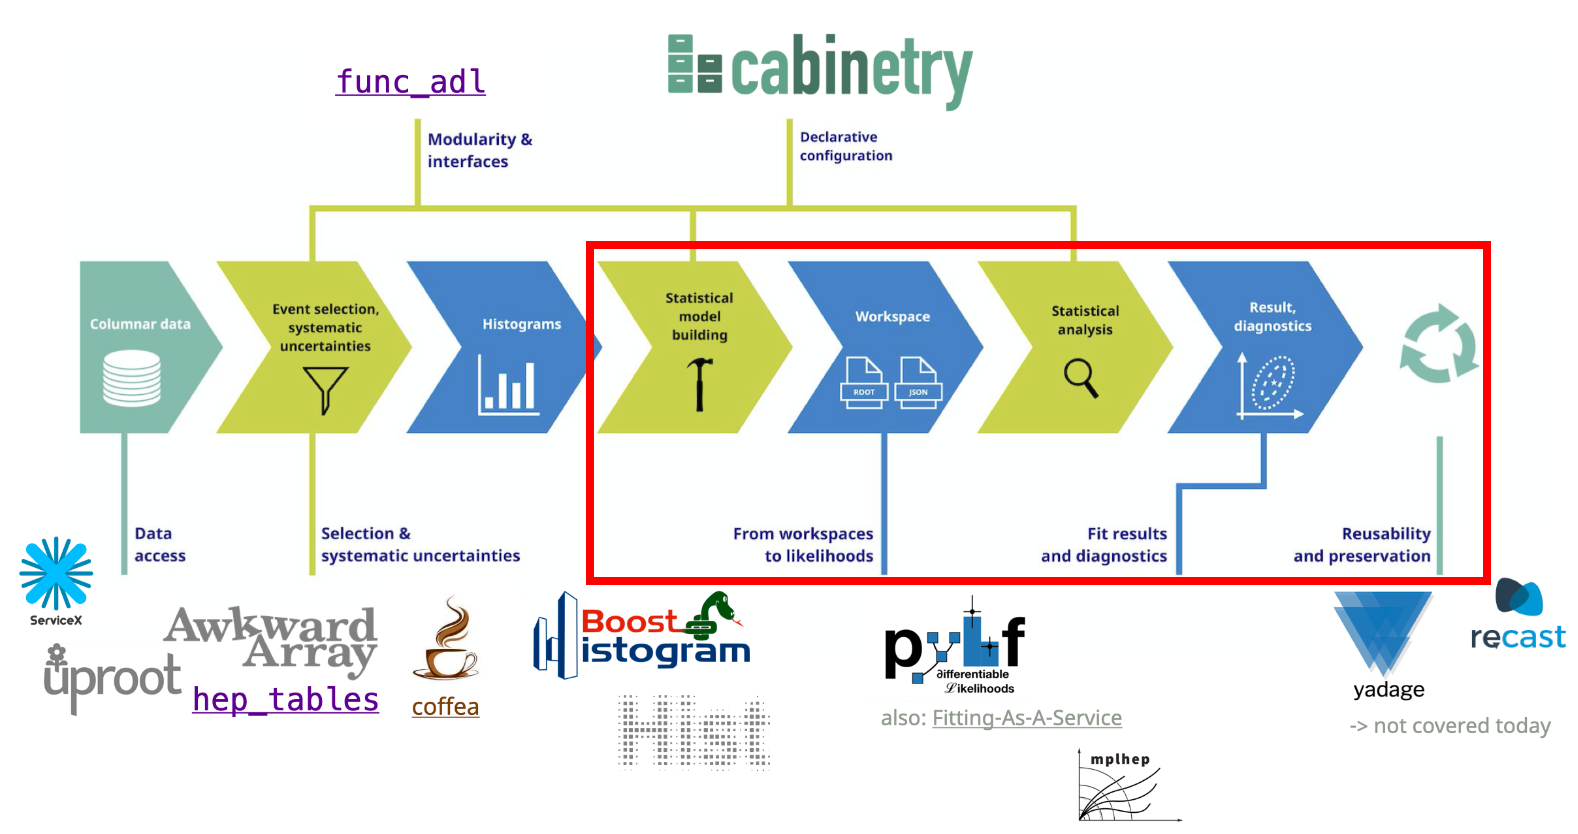
\includegraphics[width=0.8\linewidth]{ecosystem.png}
    \caption{Overview of the IRIS-HEP Analysis Systems pipeline for analysis in the HL-LHC era.
The red outline indicates the areas of the pipeline in which \pyhf{} is used either directly or as an underlying library.}
    \label{fig:analysis-systems-pipeline}
\end{figure}
